\documentclass{article}

\usepackage{tikz}
\usepackage{circuitikz}
\usepackage[utf8]{inputenc}
\usepackage[english,bulgarian]{babel}
\usepackage{graphicx}
\usepackage{caption}

\title{Приложение на математиката за моделиране на реални процеси. Моделиране на неврон.}
\author{Тонка Желева \and Васил Пашов}

\begin{document}

\maketitle
\newpage

\tableofcontents
\newpage
\title{TO DO}
\begin{enumerate}
    \item Науката за невроните и приложение
    \item Структура на неврона
        \begin{enumerate}
            \item Обобщено устройство на неврона
            \item Синапси
        \end{enumerate}
    \item Мембрана на неврона
    \item Аксонът на Ходжкинс-Хъксли
        \begin{enumerate}
            \item Изравняване на напрежението (Voltage Clamping)
        \end{enumerate}
    \item Извеждане на математическия модел и метод за решаване
    \item Програмна реализация на математическия модел и анимация
\end{enumerate}

\section{Науката за невроните и приложение}

Мозъкът, намиращ се в черепната кухина, е част от централната нервна ссистема. Той е основният орган, който обработва всички съзнателни и
несъзнателни стимули, чувства,  познания и памет. Също така е отговрен за контролирането на множество други органи. Основната градивна
единица на мозъка е неврона. Човешкия мозък съдържа около   неврона. Невронните клетки приемат, обработват и изпращат нервния импулс.
Животните реагират на външни въздействия, използвайки невроните.  Например при заплаха от изгаряне, рецепторите за топлина на сензорен
неврон осъществяват връзка със стимула и изпращат информация до интер-неврон в централната нервна система. От там мото-неврон изпраща
отговорът до скелетните мускули, които карат тялото да се отдръпне. В основата на извършването на този процес стои невротрансмисията, която
се извършва във всични неврони в човешкото тяло. Невроните пренасят тази информация чрез промени в електричесния потенциал на мембраната.

Пример за заболяване, пряко свързано с протичането на нервните импулси, е множествената склероза. Множествената склероза засяга способността на нервните клетки на главния и гръбначния мозък да комуникират помежду си.Аксоните са обгърнати от изолираща субстанция – миелин. При МС собствената имунна система атакува и унищожава миелиновото покритие. Когато миелинът бъде загубен, аксоните не могат да провеждат ефективно сигналите. Въпреки обширните познания за протичането и прогресирането на заболяването, пусковият механизъм остава засега неизвестен. Не съществува познато лекарство за множествена склероза. Лечението е насочено към възстановяване на функциите след пристъп, превенция от нови пристъпи и предотвратяване на трайната инвалидизация.

\section{Устройство на неврона}
Тъй като електрическите сигнали са в основната на преноса на информация в нервната система, е необходимо да разберем как се пораждат и пренасят тези сигнали. Проблем при невроните представляват акосните, тъй като те са дълги и не са добри проводници. За да се компесира този недостатък невроните развиват система, която им помага да пренасят сигнали на голямо разтояние, въпреки техните лоши електрически характеристики.  Електрическите сигнали, възпроизведени от тази система се наричат акционни потенциали или импулси. Ключова роля в тази система заема клетъчната мембрана.


\textbf{аксон} - най-издълженият израстък на неврона, чиято дължина може да надхвърли десетки хиляди пъти диаметъра на клетъчното тяло. Аксонът
извежда нервните импулси от клетъчното тяло, пренасяйки информация до друга клетка. Нервните импулси са еднопосочни в аксонът, но невронът
може да получи информация под формата на протеини които се придвижват от синапса до клетъчното ядро. Много неврони имат само един аксон, но
той се разклонява в много направления и така прави възможна комуникацията с много клетки. 

\textbf{клетъчна мембрана} - плазмената мембрана е изградена от двоен липиден слой. В него са вградени мембранните белтъци, които изпълняват важни функции: транспортни, енергетични, структурни, сензорни. Строежът, съставът и формата на една мембрана не са постоянни, а динамично се изменят според функциите, които трябва да извършва и според състоянието на клетката.

\section{Общо описание на процеса на невротрансмисия}
Навлизащите сигнали могат да бъдат стимулиращи, които възбуждат неврона т.е. генерират електрически импулс или инхибиращи - предотвратят неврона от активиране. Повечето неврони получават сигнали през своите дентритни дървета. Един неврон може да има повече от една група дендрити, чрез които получава хиляди сигнали. Дали един неврон ще е активиран зависи от сумата на възбуждащите и възпиращите сигнали.
В своя край аксонът се разклонява в образования наречени терминали. Тези акосанални терминали осъществяват връзката с клетките, които трябва да получат сигнала. Присинаптичен неврон, постсинаптичен неврон. В повечето синапси информацията се предава чрез химически съобщения, наречени невротрансмитери. Когато акционният потенциал преминава по аксона и достига аксонния терминал, той отключва освобождаването на невротрансмитер в синаптичната цепнатина.

Невротрансмитърите прекосяват синапса и се смесват с мембранните рецептори на постсинаптичната клетка, предавайки стимулиращия или инхибиращ сигнал. Химическият синапс е специално съединение между два неврона, което позволява те да си комуникират без да са физически свързани. Невронът завършва с малко разширение, наречено присинаптичен терминал. От другата страна на неврона имаме постсинаптичен терминал. Акционният потенциал кара калциевите йонни каналчета на терминала да се отворят. Невротрансмитерите се освобождават чрез екзоцитоза. Те бързо дифузират в синаптичната празнина. Когато достатъчно калиеви каналчета се отворят посинаптичната празина се деполяризира и актион потенциала продължава по неврона.Това води до деполяризация (смяна на поляритета), отвътре клетката се зарежда положително, следва реполяризация и се получава акционен потенциал. Промените в мембраната  са израз на възбуждане и се наричат възбуждащ постсинаптичен потенциал. Големината на постсинаптичния потенциал зависи от количеството на отделения медиатор и от чувствителността на постсинаптичната мембрана.

\section{Моделиране на електрическите свойства на клетъчната мембрана}
Всички животински клетки са обградени от мембрана, състояща се от двоен липиден слой, в който са вградени протеини. Мембраната служи както за изолатор така и за дифузионна бариера за движението на йоните. Транспорни протеини (помпи) изтласкват навън йони, а йонните каналчета позволяват на йоните прекосят мембраната и да навлязат в клетката. 

Мембранният потенциал педставлява разликата между вътрешността на клетката и извънклетъчната среда.

Понеже има разлика в потенциалите в клетъчната мембрана, казваме, че мембраната е поляризирана:
\begin{itemize}
  \item aко мембранният потенцял стане по-позитивен спрямо равновесния потенциал, казваме, че мембраната е дополяризирана.
  \item aко мембранният потенциал стане по-негативен от равновесния потенциал, казваме, че мембраната е хиперполяризирана.
\end{itemize}

Всички електрически сигнали, които използват невроните за комуникация, представляват деполяризация или хиперполяризация на равновесния мемранен потенциал.

\subsection{Равновесен мембранен потенциал}

Равновесния потенциал се определя от неравното разпределение на йони между вътрешността и външната среда на клетката и различната пропускливост на клетката към различните видове йони.

\subsection{Видове йони, намиращи се в клетката}

В невроните и обграждащата ги течност, най-често срещани са следните йони:
\begin{itemize}
  \item положително заредени -натриеви и калиеви
  \item отрицателно заредени -хлоридни
\end{itemize}

В повечето неврони К+ йони са с по-голяма концентрация във вътрешността на клетката. Обратно, обикновено, Na+ и Cl- са с по-голяма концентрация извън клетката.

\subsection{Как йоните прекосяват мембраната}

Тъй като са заредени, йоните не могат да преминат директно през хидрофобните липидни области на мембраната. Вместо това те трябва да използват специализираните протеини, които образуват хидрофилен тунел през мембраната. Някои от каналчетата са отворени, когато неврона е в покой, а други се активирит при въздействие от сигнал. Някои йонни каналчета са избрителни спрямо пропускливостта на различните видове неврони, съответно се наричат калиеви и натриеви каналчета. При невроните равновесният потенциал се влия главно от движението на К+ през калиевите каналчета.

\vspace{5mm} %5mm vertical space


\section{Акционен потенциал}
Когато входен сигнал достигне тялото на клетката, невронът ще ускори рапространяваща се промяна в мембранния потенциал. Преминаващата вълна на електричесво се нарича акционен потенциал. Акционните потенциали преминават с константна скорост от около 100m/s и с константна честота. 
В спокойно състояние невроните имта равновесен потенциал от -60 до -70 миливолта. Това означава, че вътрешната част на клетката е отрицателно заредена.

\subsection{Цикъл на акционния потенциал}

Акциноният потенциал се задейства, когато деполяризацията увеличи мембранния волтаж, така че де премине граничната стойност, която е обикновено -55 миливолта. При достигането на тази граница, N+ каналчета, зависещи от волтажа, се отварят и позволяват на натриевите йони да навлязат в клетката. Този поток от натриеви йони увеличава мембранния потенциал много бързо, докато той достигне +40 миливолта. След кратък период от време, натриевите каналчета се самодективират, спирайки навлизането на натрия. Множество калиеви каналчета, зависещи от волтажа, се отварят позволявайки на калия да излезе извън клетката. Това бързо намалява мембранния потенциал, връщайки го обратно в нормалното му равновесно положение. Калиевите каналчета остават отворени по-дълго време, но в крайна сметка те се затварят и мембранни потенциал се стабилизира. Натриевите каналчета се връщат в нормалното си състояние, затворени, но очакващи стимулиращо напрежение. Така цикълът на акционния потенциал може да започне отново.

\subsection{Предаване на сигнала от акционния потенциал}

Потенциала на аксона може да преминава само в една посока - от тялото на клетката към терминала на аксона. Когато една област от мембраната e подложена на въздействието на акционния потенциал, много N+ йони, навлизат в тази част на клетката. Тези йони се разпръзкват във вътрешността на клектака и могат да деполяризират съседни области на мембраната, подтиквайки отварянето на натриевите каначлчета и предизвиквайки протичането на акционен потенциал в тази част.

\subsection{Мембраната като електрическа верига}

За да можем да моделираме електрическите свойства на мембраната, ще ги представим като елементи в еквилентната и електрическа схема. Хидрофилните участатъци на молекулите, изграждащи клетъчната мембрана, притежават способността да се йонизират, а хидрофобните участаци образуват централен диелектричен слой. Така можем да определим клетъчната мембрана като кондензатор, който се характеризира с електричен капацитет. Капацитетът на един кондензатор, c, расте с увеличаване на площта на плочите, A, и намалява с увеличаване на разстоянието между тях, d. В биологичните мембрани дебелината на хидрофобния участък от липидния бислой е много малка – около 2.5 nm. Това определя много висока стойност на мембранния капацитет – близо до 1 /микрофарада/ .  Използваме следната формула за изчисляване на “специфичния капацитет” /тук слагаме формула/. Натрупването на заряд от двете страни на мембраната, получен от разликата в концентрацията на йоните, предизвиква потенциална разлика между вътрешната и външната част на клетката. Тя може да бъде измерена с формулата /тук слагаме формулата/. Тъй като капацитета на мембраната е голям, дори натрупването на малък заряд от двете и страни води до голяма потенцилна разлика./тук има за довършване/ 

\section{Аксонът но Ходжкинс-Хъксли}
\subsection[Изравняване на напрежението]{Изравняване на напрежението\footnote{Voltages Clamping}}
    За да можем да изследваме напълно някое свойство на даден предмет, трябва да можем да го контролираме процесите, в които това свойство
    се проявява.  Един от най - важните ппроцеси за нас е процесът по обмяна на вещества.  Обмяната на вещества от своя страна, обаче влияе
    на напрежението в неврона, което от своя страна влияе на обмяната на веществана. Виждаме, че се получава цикличен процес, който се
    изследва много трудно. За наше щастие съществува начин, по който да фиксираме напрежението в неврона. Този метод са използвали Ходжкинс
    и Хъксли. Нека разгледаме следната схема.
    \begin{center}
        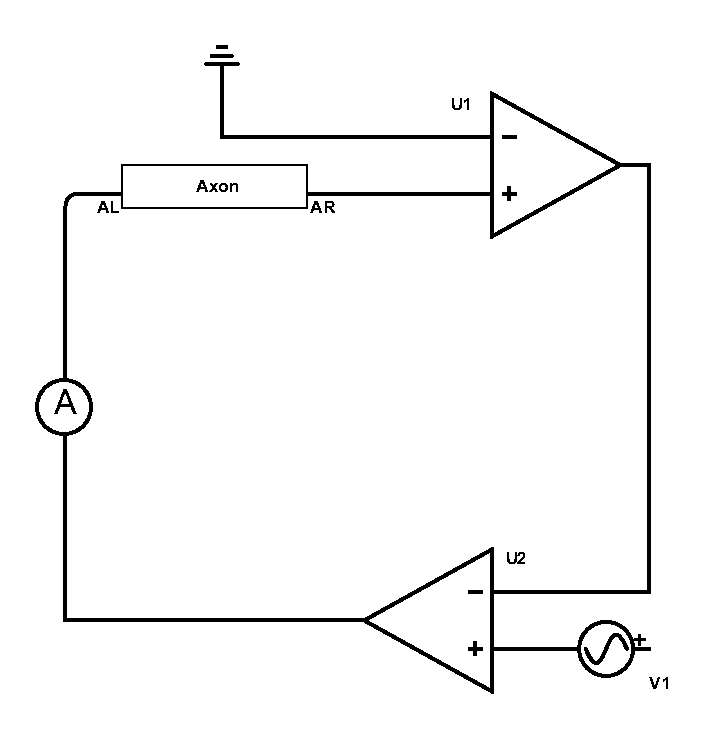
\includegraphics{./schemas/voltage-clamp.pdf}
    \end{center}
    През аксона е прокаран дълъг и тънък проводник, свързан с положителния вход на усилвател с коефициент 1. Отрицателният вход на усилвателя
    е заземен (или е свързан с течност като тази в която се намира неврона). По този начин усилвателя предава ток с напрежение $V_n$ равно на
    напрежението в самия неврон. Този ток се подава като отрицателен вход на друг усилвател с коефициент 1. На положителния вход на този
    усилвател се подава ток с напрежение двойно на желаното равновесно напрежение $V_d$. Този ток през амперметър и след това се подава в
    другия край на аксона. По точи начин ако $V_n > 2V_d$ в точката $AL$ напрежението ще бъде по - ниско от нормалното за акосна, за да се
    компенсира това положителните частици ще се насочат в тази посока, намаляки напрежението в аксона. Напрежението ще намалява клонейки към
    $V_n$ и когато стане равно на $V_n$ токът, излизащ от усилвател $U_2$ ще бъде с напрежение $U_d$, като така се получава равновесие в
    системата.
\subsection{Извеждане на математическия модел}
    Ще разглеждаме невронът като дългъг и тънък кабел. Това означава, че напрежението/токът, по него ще зависи само от една пространствена
    променлива -- $x$. Нека с $j\left(x, t\right)$ означим потока на електрически заряди в точка $x$. С други думи, $j\left(x, t\right)$ e
    скоростта, с която преминава електрическя заряд през точката, $x$. Нека сега разгледаме един, достатъчно малък интервал от неврона
    $\left[\xi, \xi+\Delta\xi\right]$:

    \begin{figure}[h!]
        \centering
        %Uncomment next line if XeTeX is used
%\def\pgfsysdriver{pgfsys-xetex.def}
\baselineskip=10pt
\hsize=6.3truein
\vsize=8.7truein
\tikzpicture[line cap=round,line join=round,>=triangle 45,x=1.0cm,y=1.0cm,scale=0.7]
\clip(-1,-5.04) rectangle (19.62,6.3);
\draw (2,-2)-- (14,-2);
\draw (2,2)-- (14,2);
\draw (6,2)-- (6,-2);
\draw (10,2)-- (10,-2);
\draw [->] (2,0) -- (6,0);
\draw [->] (10,0) -- (14,0);
\draw [->] (8,0) -- (8,4);
\fill [color=black] (6,-2) circle (1.5pt);
\draw[color=black] (5.96,-2.28) node {$\xi$};
\fill [color=black] (10,-2) circle (1.5pt);
\draw[color=black] (10.7,-2.28) node {$\xi+\Delta\xi$};
\draw[color=black] (4.32,0.22) node {j($\xi$,t)};
\draw[color=black] (12.5,0.24) node {j($\xi+\Delta\xi$,t)};
\draw[color=black] (8.82,2.72) node {i(x,t)};
\endtikzpicture


        \caption{}
    \end{figure}

    От закона за запазване на електрическия заряд знаем, че сумата от електричните заряди в една затворена система (система, която не обменя
    частици с околната среда) се запазва. Това означава, че изменението в интервала, който разглеждаме е равно на разликата между потока във
    входната точка и потока в изходната точка. За да получим общото изменение, трябва да съмираме изменението във всяка точка от интервала,
    това води до следното уравнение:
    \begin{equation}
        j\left(\xi,t\right) - j\left(\xi + \Delta\xi, t\right) = \int_{\xi}^{\xi + \Delta\xi} j\left(x, t\right) dx
    \end{equation}
\end{document} 
